\chapter{Gesten}
\label{chap:Gesten}
% Einf\"uhrung
Gestik spiegelt einen wesentlichen Teil unseres Alltags dar. Als Teil der nonverbalen Kommunikation dienen sie zum Ausdruck von Emotionen, zur \"Ubermittlung von Einstellungen, zur Darstellung von Pers\"onlichkeitseigenschaften oder Modulation einer verbalen Nachricht, so Archer und Akert~\cite{bib:archer}. 
\newline
Nachdem bereits die wissenschaftliche Definition einer Gesten nach Kurtenbach und Hulteen in Kapitel~\ref{chap:Einleitung} aufgef\"uhrt wurde und einf\"uhrende Beispiele erl\"autert wurden, werden hier Gesten tiefgehender betrachtet.

\section{Kategorisierung}
Gesten k\"onnen isoliert, oder im Zusammenhang mit einem externen Einfluss oder Objekt existieren. Ein bekanntes Beispiel f\"ur isolierte oder auch freigestellte Gesten, ist die Zeichensprache. In Bezug auf Objekte gibt es eine gro\ss e Bandbreite an m\"oglichen Gesten.
\newline
Daher wurden Gesten in Klassen eingeteilt, um diese besser unterscheiden zu k\"onnen. Die Klassifikation nach Cadoz~\cite{bib:cadoz}, die Gesten nach deren Funktion gruppiert, defniniert drei Typen:
\begin{itemize}
\item \textit{\glslink{Semiotik}{semiotisch}}: Diejenigen Gesten, die aussagekr\"aftige Informationen kommunizieren
\item \textit{\glslink{Ergo}{ergodisch}}: Diejenigen Gesten, die genutzt werden, um das reale Umfeld zu manipulieren und Gegenst\"ande  zu erstellen
\item \textit{\glslink{Epistemik}{epistemisch}}: Diejenigen Gesten, die genutzt werden, um von der Umwelt durch taktile und haptische Erkundung zu lernen
\end{itemize}
Dar\"uber hinaus werden diese Klassen weiter unterteilt. Das Augenmerk dieser Arbeit liegt auf den semiotischen Gesten. Innerhalb dieser Kategorie liefert Mulder~\cite{bib:Mulder} eine weitere Sammlung an verschiedenen Klassifikationen.
\newline
Da der Fokus dieser Arbeit auf der \gls{MCI} liegt, werden vorrangig sogenannte \textit{empty handed} semiotische Gesten betrachtet. Diese k\"onnen entsprechend ihrer Funktionalit\"at weiter unterteilt werden. Rime und Schiaratura~\cite{bib:rime} beschreiben folgende Taxonomie:
\begin{itemize}
\item \textit{symbolische Gesten}: Dabei handelt es sich um Gesten, die innerhalb eines bestimmten Kulturkreises, eine allgemeing\"ultige Bedeutung erlangt haben. Das \enquote{Daumen Hoch}-Zeichen, w\"ahre ein solches Beispiel
\item \textit{\glslink{Deixis}{deiktische} Gesten}: Unter dieser Kategorie fallen Gesten des Zeigens oder der Richtungsweisung. Diese stehen meist in einem Kontext, wie \enquote{Lege das hier hin}
\item \textit{\glslink{Ikoni}{ikonische} Gesten}: Darunter fallen Gesten, die Informationen \"uber Form, Gestalt und Auspr\"agung eines bestimmten Gegenstandes oder einer Handlung
\item \textit{\glslink{Panto}{pantomimische} Gesten}: Dies sind Gesten, die typischer Weise die Nutzung eines nichtgegenw\"artigen Gegenstandes oder Werkzeugs wiederspiegeln. W\"ahrend der Mimik einer Aktion wird dabei eine pantomimische Geste gemacht
\end{itemize}
Baudel und Beaudouin-Lafon~\cite{bib:baudel} zeigen einige Vorteile der Nutzung von symbolischen Gesten zur Interaktion auf:
\begin{itemize}
\item \textit{Nat\"urliche Interaktion}: Gesten sind eine selbstverst\"andliche Form der Interaktion und einfach zu verwenden
\item \textit{Knapp und Ausdrucksstark}: Eine Geste \"ubermittelt genug Information, um Befehl und Paramter zu liefern
\item \textit{Direkte Interaktion}: Einzelne K\"orperteile, insbesondere die Hand, als Eingabeger\"ate machen weitere Signalgeber zwischen Eingabe und Empf\"anger obsolet
\end{itemize}
Nat\"urlich bergen diese auch Nachteile. So k\"onnen symbolische Gesten auf Dauer anstrengend und aufw\"anding werden. Ein Nutzer ben\"otigt in aller Regel Training und ein detailiertes Wissen \"uber Anwendung und Funktion der Gesten, bevor er in der Lage ist, die Anwendung mittels symbolischen Gesten zu bedienen. Je weiter die Anzahl der Gesten und deren Komplexit\"at steigt, desto schwieriger wird es, sich an bestimmte Gesten zu erinnern.
\newline
Weiter stellt sich ein Segmentierungsproblem, dahingehend, dass eine Bewegungsdetektion in aller Regel, den gesamten Verlauf einer Handbewegung, oder die eines anderen K\"orperteils erfasst und die eigentliche Geste nur einen Ausschnitt dieses kontinuierlichen Signalstroms darstellt.
\newline
Es ist daher wichtig, Gesten, die in einer Anwendung verwendet werden sollen, so zu modellieren, dass sie einfach auszuf\"uhren sind, eine angemessene Unterscheidung zwischen diversen Gesten vorhanden ist und diese sich m\"oglichst nahe an nat\"urlichen Bewegungen orientieren.

% jede Geste genau beschreiben - grafik dazu \ldots konzept \ldots realbild von kinect
% hmm modell, genaue beschreibung, stati, \"ubergangsmatrix, zahlen zahlen zahlen
% verkn\"upfung mit aktion f\"ur roboter
\section{Gesten in der Anwendung}

Nachdem bereits in Abschnitt~\ref{subsec:Analyse} die Anforderungen an Gesten ausgef\"uhrt wurden, werden hier die daraus entwickelten Gesten aufgef'\"uhrt. Dabei werden alle grundlegenden Vorgaben f\"ur ein \gls{MCI} aus Abschnitt~\ref{subsec:MCI} ber\"ucksichtigt und die zu entwerfenden Gesten auf Basis der oben beschriebenen Kategorie der \glslink{Semiotik}{semiotischen} Gesten modelliert.

\subsection{Kreisbewegung}
Ein abstrakter Robot, ist in aller Regel in der Lage, sich im Stand vollst\"andig um seine eigene Achse zu drehen. Dies ist eine hilfreiche Funktion zur Steuerung eines solchen Ger\"ats. Betrachtet man diese Drehung, so findet im Grunde eine Kreisbewegung statt. Um eine intuitive Assoziation zwischen dieser Drehung und der daf\"ur zu verwendeten Geste herzustellen, wird zur Durchf\"uhrung dieser Geste, eine Kreisbewegung verlangt. Das hei\ss t bildlich gesprochen, dass der Bediener mit seinen H\"anden einen Kreis in die Luft zeichnen muss, um die Geste auszuf\"uhren.
\newline
Die Ausf\"uhrung dieser Bewegung ist intuitiv und ohne nennenswerten Trainingsaufwand anwendbar.

\subsubsection{Fachliche Aspekte}
Die Kreisbewegung ist eine ikonische Geste, da sie die Form eines Kreises wiedergibt. 

\subsubsection{Technische Aspekte}


\begin{figure}[htb]
\centering
\begin{tikzpicture}[
    scale=4,
    axis/.style={very thick, ->, >=stealth'},
    every node/.style={color=black},
    auto,
    ]
    % axis
    \draw[axis] (-1,0)  -- (1.1,0) node(xline)[right]
        {$x$};
    \draw[axis] (-0.5,-0.5) -- (0.5,0.5) node(zline)[above] {$z$};
    % Lines
    \draw[axis] (0,-1) -- (0,1.1) node(yline)[above] {$y$};
    % Lines

\filldraw[fill=gray!5] (0,0) circle (0.8);

\fill  (0,0.8) circle (.4pt) node[above right]{$S_1$};
\fill  (0.62,0.5) circle (.4pt) node[above right] {$S_2$};
\fill  (0.8,0) circle (.4pt) node[above right] {$S_3$};
\fill  (0.62,-0.5) circle (.4pt) node[ right] {$S_4$};
\fill  (0,-0.8) circle (.4pt) node[above right] {$S_5$};
\fill  (-0.5,-0.62) circle (.4pt) node[above right] {$S_6$};
\fill  (-0.8,0) circle (.4pt) node[above right] {$S_7$};
\fill  (-0.62,0.5) circle (.4pt) node[right] {$S_8$};

\draw [<->, thick] (0.05, 0.95) arc (90:-265:0.95);
\end{tikzpicture}
\caption[Abstrakte Darstellung einer Kreisbewegung im Koordinatensystem inklusiver ihrer 8 Zustandspunkte]{Abstrakte Darstellung einer Kreisbewegung im Koordinatensystem inklusiver ihrer 8 Zustandspunkte}
\label{fig:Circle_ideal}
\end{figure}

In einem \acrshort{HMM} wird diese Bewegung durch acht Zust\"ande modelliert. Abbildung~\ref{fig:Circle_ideal} zeigt ein ideales Bild dieser Geste mit ihren acht Zust\"anden.

\begin{figure}[htb]
\centering
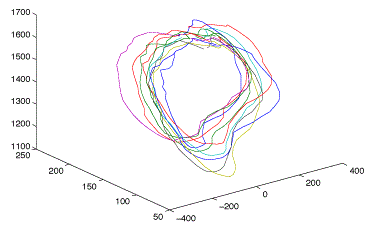
\includegraphics[width=0.5\textwidth]{img/gesture/gesture_circle_real.png}
\caption[Darstellung von Kreisbewegungen im Koordinatensystem die aus realen Trainingsdaten stammen]{Darstellung von Kreisbewegungen im Koordinatensystem die aus realen Trainingsdaten stammen\protect{\footnotemark[1]}}
\label{fig:Circle_reall}
\end{figure}

Diese acht Zust\"ande bilden ein Mittelma\ss dar, um auf der einen Seite kein unterdimensioniertes \gls{HMM} aufzustellen, auf der anderen Seite, aber gen\"ugend Spielraum f\"ur die Akzeptanz von Kreisbewegungen einer etwas ungenauen Form zuzulassen. Abbildung~\ref{fig:Circle_real} zeigt mehrere solcher Kreise, die aus Trainingsdaten ermittelt worden sind.

\footnotetext[1]{Quelle:~\href{http://www.creativedistraction.com/demos/gesture-recognition-kinect-with-hidden-markov-models-hmms/}{\enquote{How to Do Gesture Recognition With Kinect Using Hidden Markov Models (HMMs)}}. creativedistraction.com. Abgerufen Januar 14, 2013}

Die \"Ubergangsmatrix $A$, f\"ur die Geste einer Kreisbewegung wird definiert, als
\begin{equation}
\mathbf{A} = 
\begin{pmatrix}
a_{11} & a_{12} & 0 & 0 & 0 & 0 & 0 & 0 \\
0 & a_{22} & a_{23} & 0 & 0 & 0 & 0 & 0 \\
0 & 0 & a_{33} & a_{34} & 0 & 0 & 0 & 0 \\
0 & 0 & 0 & a_{44} & a_{45} & 0 & 0 & 0 \\
0 & 0 & 0 & 0 & a_{55} & a_{56} & 0 & 0 \\
0 & 0 & 0 & 0 & 0 & a_{66} & a_{67} & 0 \\
0 & 0 & 0 & 0 & 0 & 0 & a_{77} & a_{78} \\
0 & 0 & 0 & 0 & 0 & 0 & 0 & a_{88} \\
\end{pmatrix} \, .
\end{equation}

Dabei ist die Wahrscheinlichkeit des \"Ubergangskoeffizienten $a_{88}$ gleich $1$. Weiter wird zur Initialisierung f\"ur die weiteren Indizes $i, j$ auf der Hauptiagonalen und der rechten Nebendiagonalen, $a_{ij} = 0,5$ gesetzt. In Trainingsdurchl\"aufen m\"ussen diese Wahrscheinlichkeiten eventuell vereinzelt angepasst werden.

\subsection{Vorw\"artsbewegung}

\subsubsection{Fachliche Aspekte}
Die Vorw\"artsbewegung ist eine deiktische Geste, da sie eine Richtungsanweisung wiedergibt. 

\subsubsection{Technische Aspekte}
\begin{figure}[htb]
\centering
\begin{tikzpicture}[
    scale=4,
    axis/.style={very thick, ->, >=stealth'},
    ]
    % axis
    \draw[axis] (-0.1,0)  -- (1.1,0) node(xline)[right]
        {$x$};
    \draw[axis] (-0.1,-0.1) -- (0.5,0.5) node(zline)[below right] {$z$};
    % Lines
    \draw[axis] (0,-0.1) -- (0,1.1) node(yline)[above] {$y$};
    % Lines

\filldraw[fill=gray!20, fill opacity=0.8] (0,0.8) .. controls (0.1,0.8) and (0.35,0.66) .. (0.48,0.48);
\filldraw[fill=gray!20,fill opacity=0.8, draw opacity = 0](0,0.8) -- (0.48,0.48) -- ( 0,0);
 \draw  (0.1,0.1) arc (90:10:0.1)  ;
\fill (0.11,0.048) circle (.2pt) ;

\fill  (0,0.8) circle (.4pt) node[above right] (a) {$S_1$};
\fill  (0.15,0.74) circle (.4pt) node[above right] {$S_2$};
\fill  (0.35,0.61) circle (.4pt) node[above right] {$S_3$};
\fill  (0.48,0.48) circle (.4pt) node[above right] {$S_4$}
 edge[pil,<->, bend right=60] (a);
\end{tikzpicture}
\caption[Abstrakte Darstellung einer Vorw\"artsbewegung im Koordinatensystem inklusiver ihrer 4 Zustandspunkte]{Abstrakte Darstellung einer  Vorw\"artsbewegung im Koordinatensystem inklusiver ihrer 4 Zustandspunkte}
\label{fig:Foward_ideal}
\end{figure}


\begin{tikzpicture}[
    scale=4,
    axis/.style={very thick, ->, >=stealth'},
    every node/.style={color=black}
    ]
    % axis
    \draw[axis] (-0.1,0)  -- (1.1,0) node(xline)[right]
        {$x$};
    \draw[axis] (-0.1,-0.1) -- (0.5,0.5) node(zline)[above] {$z$};
    % Lines
    \draw[axis] (0,-0.1) -- (0,1.1) node(yline)[above] {$y$};
    % Lines

\filldraw[fill=gray!5,fill opacity=0.8] (0,0.8) .. controls (0.09,0.78) and (0.3,0.66) .. (0.48,0.48);
\filldraw[fill=gray!5,fill opacity=0.8, draw opacity = 0] (0,0.8) -- (0.48,0.48) -- (0,0);
 \filldraw[fill=gray!20,fill opacity=0.8]  (0,0) -- (0.5,0.3) arc (0:10:1) ;
    \node[] at (35:0.7)  {$\theta$};

\draw[dashed] (0,0.8) .. controls (0.09,0.78) and (0.3,0.66) .. (0.5,0.3);



\fill  (0,0.8) circle (.4pt) node[above right] (a){$S_1$};
\fill  (0.15,0.74) circle (.4pt) node[above right] {$S_2$};
\fill  (0.35,0.61) circle (.4pt) node[above right] {$S_3$};
\fill  (0.48,0.48) circle (.4pt) node[above right] {$S_4$};
\fill  (0.49,0.4) circle (.4pt) node[below left] {$S_5$};
\fill  (0.5,0.3) circle (.4pt) node[right] {$S_6$}
 edge[pil,<->, bend right=120] (a);
\end{tikzpicture}

\begin{tikzpicture}[
    scale=4,
    axis/.style={very thick, ->, >=stealth'},
every node/.style={color=black}
    ]
    % axis
    \draw[axis] (-0.1,0)  -- (1.1,0) node(xline)[right]
        {$x$};
    \draw[axis] (-0.1,-0.1) -- (0.5,0.5) node(zline)[above] {$z$};
    % Lines
    \draw[axis] (0,-0.1) -- (0,1.1) node(yline)[above] {$y$};
    % Lines

\draw (0,0.8) .. controls (0.09,0.78) and (0.3,0.66) .. (0.48,0.48);
 \filldraw[fill=gray!20,fill opacity=0.8]  (0,0) -- (0.5,0.3) arc (0:10:1) ;
    \node[] at (35:0.7)  {$\theta$};

\draw[dashed] (0,0.8) .. controls (0.09,0.78) and (0.3,0.66) .. (0.5,0.3);

\fill  (0.48,0.48) circle (.4pt) node[above right] (a){$S_1$};
\fill  (0.49,0.4) circle (.4pt) node[below left] {$S_2$};
\fill  (0.5,0.3) circle (.4pt) node[right] {$S_3$}
 edge[pil,<->, bend right=80] (a);
\end{tikzpicture}

\begin{tikzpicture}[
    scale=4,
    axis/.style={very thick, ->, >=stealth'},
every node/.style={color=black}
    ]
    % axis
    \draw[axis] (-0.1,0)  -- (1.1,0) node(xline)[right]
        {$x$};
    \draw[axis] (-0.1,-0.1) -- (0.5,0.5) node(zline)[above] {$z$};
    % Lines
    \draw[axis] (0,-0.1) -- (0,1.1) node(yline)[above] {$y$};
    % Lines

\filldraw[fill=gray!20, fill opacity=0.8] (0,0.8) .. controls (0.09,0.78) and (0.3,0.66) .. (0.5,0.3);
\filldraw[fill=gray!20,fill opacity=0.8, draw opacity = 0](0,0.8) -- (0.5,0.3) -- ( 0,0);
\draw[dotted] (0,0.8) .. controls (0.09,0.78) and (0.3,0.66) .. (0.48,0.48);
 \draw  (0,0) -- (0.5,0.3) arc (0:10:1) ;
    \node[] at (35:0.7)  {$\theta$};


\fill  (0,0.8) circle (.4pt) node[above right] (a){$S_1$};
\fill  (0.17,0.7) circle (.4pt) node[above right] {$S_2$};
\fill  (0.35,0.53) circle (.4pt) node[above right] {$S_3$};
\fill  (0.5,0.3) circle (.4pt) node[below right] {$S_4$}
 edge[pil,<->, bend right=80] (a);
\end{tikzpicture}



\subsection{Haltesignal}

\subsubsection{Fachliche Aspekte}
Das Haltesignal ist eine ... Geste, da sie eine Richtungsanweisung wiedergibt. 

\subsubsection{Technische Aspekte}
\subsection{Enriegeln --- Blockieren}

\subsubsection{Fachliche Aspekte}
Das Enriegeln --- Blockieren ist eine ... Geste, da sie eine Richtungsanweisung wiedergibt. 

\subsubsection{Technische Aspekte}

\begin{tikzpicture}[
    scale=4,
    axis/.style={very thick, ->, >=stealth'},
    every node/.style={color=black},
node distance=1cm, auto,
    ]
    % axis
    \draw[axis] (-0.1,0)  -- (1.1,0) node(xline)[right]
        {$x$};
    \draw[axis] (-0.1,-0.1) -- (0.5,0.5) node(zline)[above] {$z$};
    % Lines
    \draw[axis] (0,-0.1) -- (0,1.1) node(yline)[above] {$y$};
    % Lines

\draw (0,0.8) --  (1,0.8);

\fill  (0,0.8) circle (.4pt) node[above right] (a){$S_1$} ;
\fill  (0.25,0.8) circle (.4pt) node[above right] {$S_2$} ;
\fill  (0.5,0.8) circle (.4pt) node[above right] {$S_3$} ;
\fill  (0.75,0.8) circle (.4pt) node[above right] {$S_4$} ;
\fill  (1,0.8) circle (.4pt) node[above right] {$S_5$}
 edge[pil,<->,  bend right] (a) ;
\end{tikzpicture}